\documentclass[12pt]{article}
\usepackage[utf8]{inputenc}
\usepackage[english]{babel}
\usepackage[dotinlabels]{titletoc}
\usepackage[nottoc,numbib]{tocbibind}
\usepackage{mathptmx}
\usepackage{amsmath, amssymb}
\usepackage{geometry, titlesec, setspace}
\usepackage{graphicx, caption}
\usepackage{hyperref, natbib}
% Journals
\newcommand{\aap}{A\&A}
\newcommand{\aj}{AJ}
\newcommand{\apj}{ApJ}
\newcommand{\araa}{ARA\&A}
\newcommand{\mnras}{MNRAS}
\newcommand{\nat}{Nature}
\newcommand{\pasa}{PASA}
\newcommand{\pasp}{PASP}
\newcommand{\physrep}{PhR}
\newcommand{\prd}{PhRvD}
\newcommand{\rpph}{RPPh}

% Page formatting
\geometry{
	left=1.25in,
	right=1.25in,
	top=1in,
	bottom=1in}
\hypersetup{
	colorlinks=true,
	citecolor=blue,
	filecolor=blue,
	linkcolor=blue,
	urlcolor=blue
}
\setlength{\footnotesep}{10pt}
\setlist{noitemsep}

% Fixing titlesec and hyperref interaction
\makeatletter
\def\ttl@useclass#1#2{%
\@ifstar
{\ttl@labeltrue\@dblarg{#1{#2}}}
{\ttl@labeltrue\@dblarg{#1{#2}}}}
\makeatother

% Image setup
\graphicspath{{figs/}}
\captionsetup[figure]{labelfont={bf}, font={small, stretch=1.3}, name={Figure}, labelsep=period}

% Section and subsection headings
\titleformat{\section}{\normalsize\bfseries\centering}{}{0em}{}
\titleformat{\subsection}{\normalsize\itshape\centering}{}{0.75em}{}
\newcommand{\nocontentsline}[3]{}
\newcommand{\tocless}[2]{\bgroup\let\addcontentsline=\nocontentsline#1{#2}\egroup}
\renewcommand{\contentsname}{Table of Contents}
\renewcommand{\abstractname}{{\normalsize\bfseries\centering{Abstract}}}
\renewcommand{\bibsection}{}

% For figures
\makeatletter
\setlength{\@fptop}{0pt plus 1fil}
\setlength{\@fpbot}{0pt plus 1fil}
\makeatother

% For formatting text and math
\let\vec\mathbf
\newcommand{\code}[1]{{\fontfamily{qcr}\selectfont#1}}
\newcommand{\red}[1]{\textcolor{red}{#1}}
\newcommand{\note}[1]{\textcolor{violet}{#1}}

% Special commands
\newcommand{\HI}{H\,\textsc{i}}
\newcommand{\OI}{O\,\textsc{i}}
\newcommand{\heraqm}{\code{hera\textunderscore qm}}
\newcommand{\herapspec}{\code{hera\textunderscore pspec}}
\newcommand{\herasim}{\code{hera\textunderscore sim}}
\newcommand{\pyuvdata}{\code{pyuvdata}}

\begin{document}
\doublespacing
\begin{center}
Environmental Systematics and the Impact on \\ 21-cm Epoch of Reionization Measurements \\
by \\
Lily Whitler \\
has been approved \\
Spring 2019 \\[0.1\textheight]

\begingroup
\renewcommand{\arraystretch}{0.7}
\begin{tabular}{p{1cm}p{3.5in}p{1cm}}
	& \centering APPROVED: & \\
	& & \\ & & \\
	& \hrulefill & \\
	& \hfill Daniel Jacobs, Director & \\
	& & \\ & & \\
	& \hrulefill & \\
	& \hfill Judd Bowman & \\
	& & \\ & & \\
	& \hrulefill & \\
	& \hfill Adam Beardsley &
\end{tabular} \\[0.075\textheight]
\begin{tabular}{p{1cm}p{3.5in}p{1cm}}
	& \centering ACCEPTED: & \\
	& & \\ & & \\
	& \hrulefill & \\
	& \hfill Dean, Barrett, The Honors College &
\end{tabular}
\endgroup
\end{center}
\thispagestyle{empty}
\newpage
\pagenumbering{arabic}

\begin{center}
	{\Large Environmental Systematics and the Impact on \\ 21-cm Epoch of Reionization Measurements} \\
	by \\
	Lily Whitler \\[0.15\textheight]
	
	A Thesis Presented in Partial Fulfillment \\
	of the Requirements for Graduation from \\
	Barrett, the Honors College \\[0.15\textheight]
	
	Committee: \\
	Daniel Jacobs, Director \\
	Judd Bowman \\
	Adam Beardsley \\[0.2\textheight]
	
	ARIZONA STATE UNIVERSITY \\
	April 2019
\end{center}
\thispagestyle{empty}

\clearpage
\pagenumbering{roman}

\begingroup
\hypersetup{
	colorlinks=true,
	citecolor=DarkBlue,
	filecolor=black,
	linkcolor=black,
	urlcolor=DarkBlue
}
\tableofcontents
\listoffigures
\listoftables
\endgroup
\newpage

\begin{abstract}
\end{abstract}

\clearpage
\pagenumbering{arabic}

\section{Introduction} \label{sec:intro}

\subsection{A Brief History of the Universe} \label{subsec:universe}

Immediately after the Big Bang, the universe was a hot plasma of fundamental particles. Now, nearly 14 billion years later, it is populated with a rich variety of \red{objects}, from massive galaxy clusters all the way down to our own solar system and its planets. The \red{evolutionary} path of the universe from the Big Bang to now, however, is not entirely clear.

In the early universe, matter was hot and ionized. Photons scattered off of free particles, rendering the universe opaque to electromagnetic radiation. This lasted until approximately 380,000 years after the Big Bang, when the universe had expanded and cooled sufficiently for electrons to become bound to atomic nuclei during recombination. When recombination was complete, photons were able to propagate freely through space, subject only to cosmological redshift. Today, we see photons from this era as the cosmic microwave background (CMB).

Immediately following the release of the CMB and lasting until several hundred million years after the Big Bang was the cosmic Dark Ages. During this era, though photons were free to propagate, no stars, galaxies, or other sources of radiation had yet formed. The only sources of information we have from the Dark Ages are CMB photons and emission from neutral hydrogen.

The transition between the Dark Ages and the subsequent Epoch of Reionization (EoR) was marked by the \red{emergence} of the first luminous sources. During the EoR, ultraviolet \red{(UV)} radiation from these objects ionized the intergalactic medium (IGM) around them. The EoR ended when the IGM was fully ionized, thus completing the final major phase change of hydrogen in the universe.

Figure \ref{fig:timeline} shows an illustration of this evolution. The \textit{Planck} satellite and its predecessors, the \textit{Cosmic Background Explorer} and \textit{Wilkinson Microwave Anisotropy Probe}, have measured the temperature and polarization anisotropies in the CMB, providing us with a wealth of information about the early universe. On the other end of cosmic history, the Hubble Deep Fields have probed some of the oldest known galaxies. However, the time in between is still lacking observational constraints. \red{I should probably have references in this section...}

\begin{figure}[tb]
	\centering
	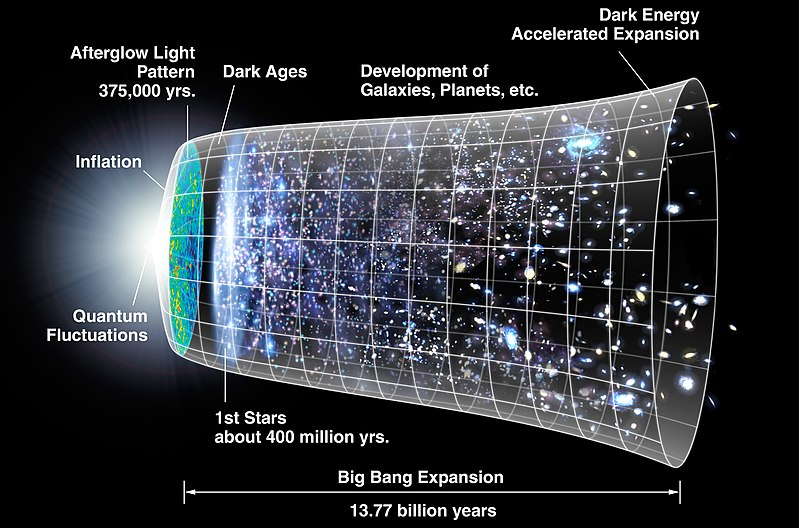
\includegraphics[width=\textwidth]{timeline.jpg}
	\caption[Timeline of the universe]{Timeline of the evolution of the universe. Image courtesy of NASA, ESA, and the Planck Collaboration.}
	\label{fig:timeline}
\end{figure}

\subsection{The Epoch of Reionization} \label{subsec:eor}

The EoR is important to understanding the processes of structure formation in the universe. The CMB exhibits density fluctuations on the order of $10^{-5}$, which gravitational instabilities eventually collapsed into

while today, we clearly have large, gravitationally bound clumps of matter (galaxies and even galaxy clusters) and voids where there are no large concentrations of mass. The process by which the small density fluctuations in the CMB evolved into the structure we see now has been explored theoretically \red{(citations?)}, but the theory encompassing the Dark Ages and the EoR has not yet been observationally \red{tested}.

\cite{furlanetto2006}

\cite{morales2010}

\cite{pritchard2012}

\subsection{The 21-cm Power Spectrum} \label{subsec:ps}

\subsection{The Hydrogen Epoch of Reionization Array} \label{subsec:hera}

\begin{figure}[tb]
	\centering
	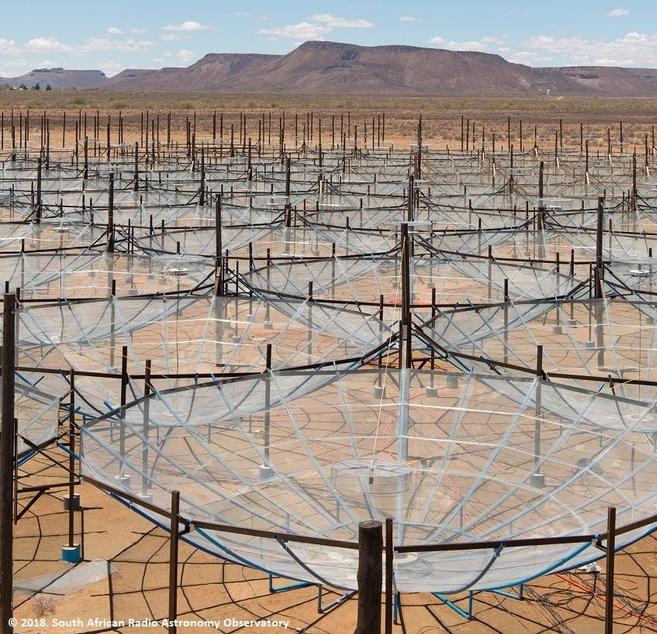
\includegraphics[width=0.75\textwidth]{hera.png}
	\caption[HERA as of late 2017 -- early 2018]{HERA as of late 2017 -- early 2018. HERA will observe large-scale structure prior to and during the EoR via the redshifted 21-cm line from the IGM. Image courtesy of the South African Radio Astronomy Observatory.}
	\label{fig:hera}
\end{figure}

The Hydrogen Epoch of Reionization Array (HERA; Figure \ref{fig:hera}) is an experiment to study the periods prior to and during the EoR \red{(from redshifts $z \sim 6 - 30$)} via measurements of the redshifted 21-cm line \citep{deboer2017}. HERA is one of several instruments designed to perform this measurement; others include the Low-Frequency Array (\red{van Haarlem et al., 2013}), the Murchison Widefield Array (\red{Tingay et al., 2013}), and in the future, the Square Kilometer Array (SKA). HERA is located in the Karoo Radio Astronomy Reserve in South Africa, a site protected by law to preserve its radio-quiet environment for radio frequency \red{experiments} like HERA.

\subsection{Radio Frequency Interference} \label{subsec:rfi}

\section{Methods} \label{sec:methods}

\subsection{RFI Excision Strategies} \label{subsec:rfi_excision}

\subsection{Calculating the Power Spectrum} \label{subsec:calc_ps}

\subsection{Modelling HERA Data} \label{subsec:modelling}

\section{Results}

\section{Conclusions}

\bibliographystyle{apj}
\bibliography{refs}
\end{document}